\documentclass{article}
\usepackage[utf8]{inputenc}
\usepackage{amsmath}
\usepackage{graphicx}
\usepackage{booktabs}
\usepackage{caption}
\usepackage{adjustbox}


\title{Informe de Análisis Exploratorio de \texttt{swiss}}
\author{
  Melani Forsythe Matos \\
  Daniela Guerrero Álvarez \\
  Rubén Martínez Rojas
}
\date{} % Sin fecha para que no aparezca
\begin{document}

\maketitle

\section{Introducción}
El dataset ``swiss'' contiene datos sobre 47 cantones suizos en 1888. Este análisis proporciona una visión detallada de las variables relacionadas con la fertilidad, la agricultura, y la educación.

\section{Descripción de las Variables}
El dataset ``swiss'' incluye las siguientes variables:
\begin{itemize}
    \item \textbf{Fertility}: Tasa de fertilidad (número de hijos por mujer).
    \item \textbf{Agriculture}: Proporción de trabajadores en agricultura.
    \item \textbf{Examination}: Proporción de jóvenes con educación secundaria.
    \item \textbf{Education}: Proporción de población con educación secundaria.
    \item \textbf{Catholic}: Proporción de población católica.
    \item \textbf{Infant.Mortality}: Tasa de mortalidad infantil (número de muertes por 1000 nacidos vivos).
\end{itemize}

\section{Análisis Descriptivo}
A continuación, se presentan los resultados del análisis descriptivo para cada variable.

\subsection{Fertility}
\begin{itemize}
    \item \textbf{Media}: 68.15
    \item \textbf{Mediana}: 69.40
    \item \textbf{Moda}: 69.40
    \item \textbf{Simetría}: -0.10
    \item \textbf{Curtosis}: -0.57
    \item \textbf{Varianza}: 125.96
    \item \textbf{Desviación Estándar}: 11.22
    \item \textbf{Rango}: 60.80
    \item \textbf{Coeficiente de Variación}: 16.48\%
\end{itemize}

\begin{figure}[h!]
\centering
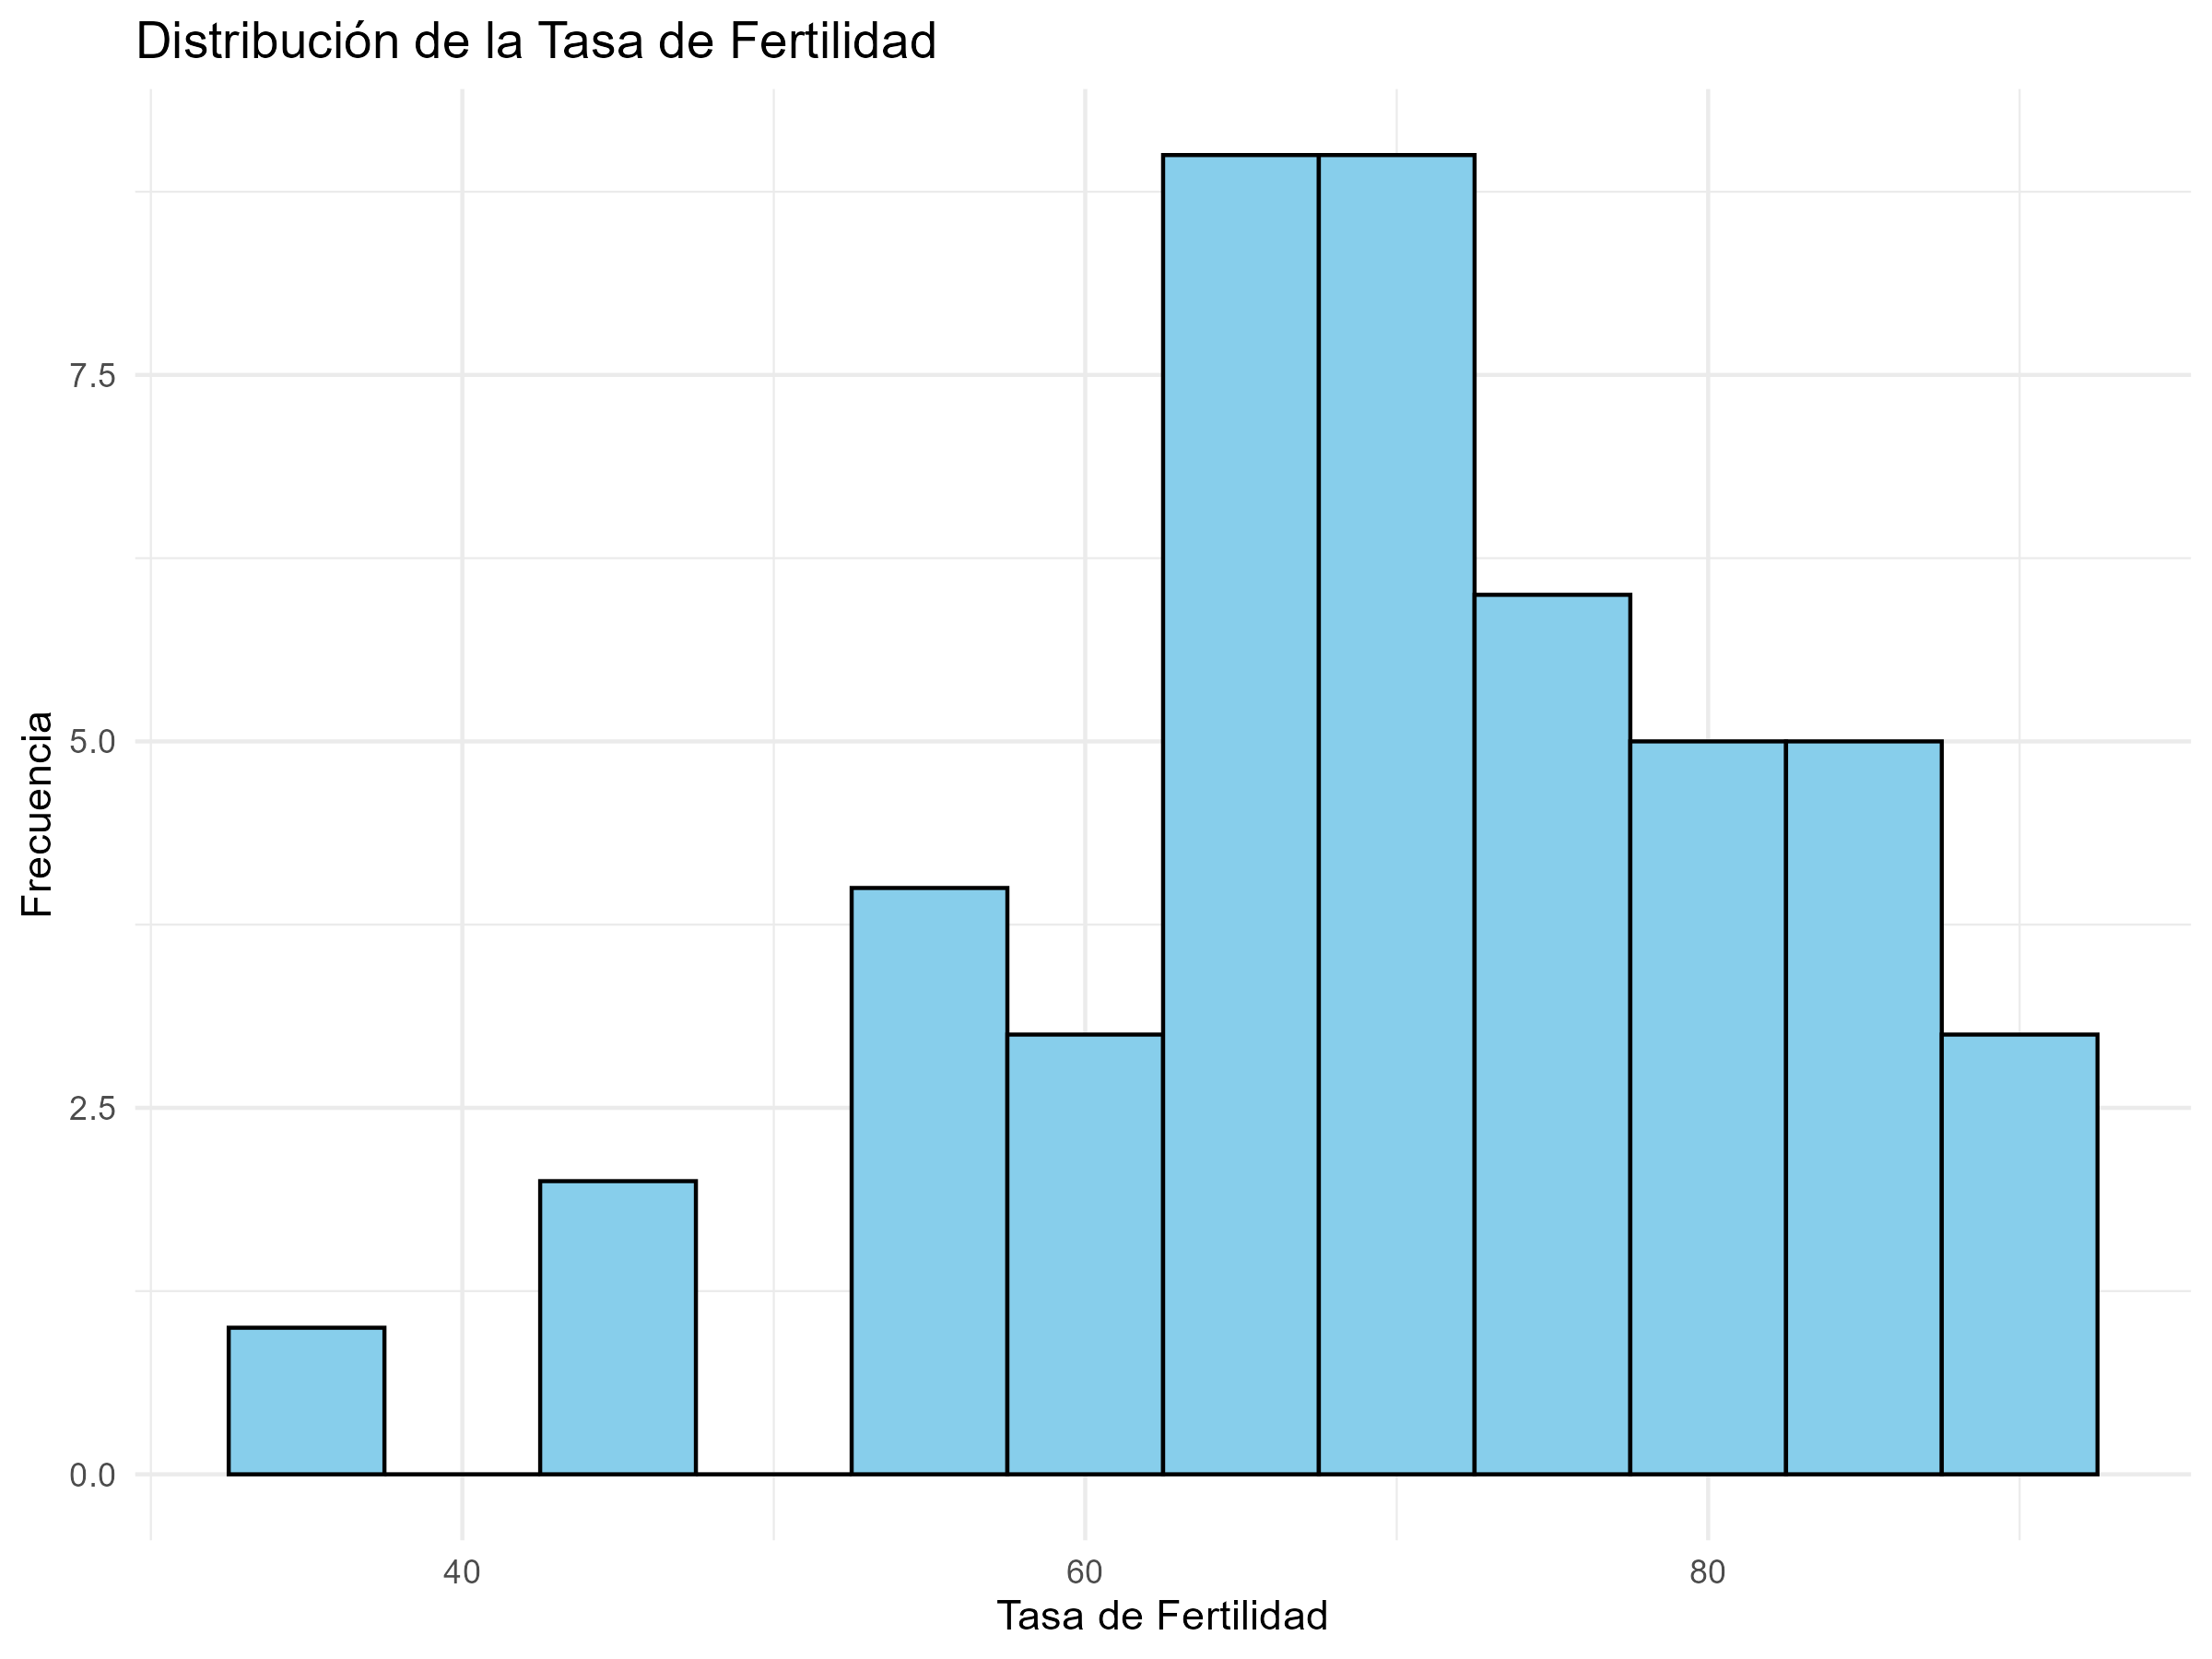
\includegraphics[width=\textwidth]{Histogramas/histogram_fertility.png}
\caption{Distribución de la Tasa de Fertilidad}
\end{figure}

\subsection{Agriculture}
\begin{itemize}
    \item \textbf{Media}: 41.47
    \item \textbf{Mediana}: 39.45
    \item \textbf{Moda}: 39.45
    \item \textbf{Simetría}: 0.29
    \item \textbf{Curtosis}: -0.66
    \item \textbf{Varianza}: 142.47
    \item \textbf{Desviación Estándar}: 11.94
    \item \textbf{Rango}: 59.30
    \item \textbf{Coeficiente de Variación}: 28.85\%
\end{itemize}

\begin{figure}[h!]
\centering
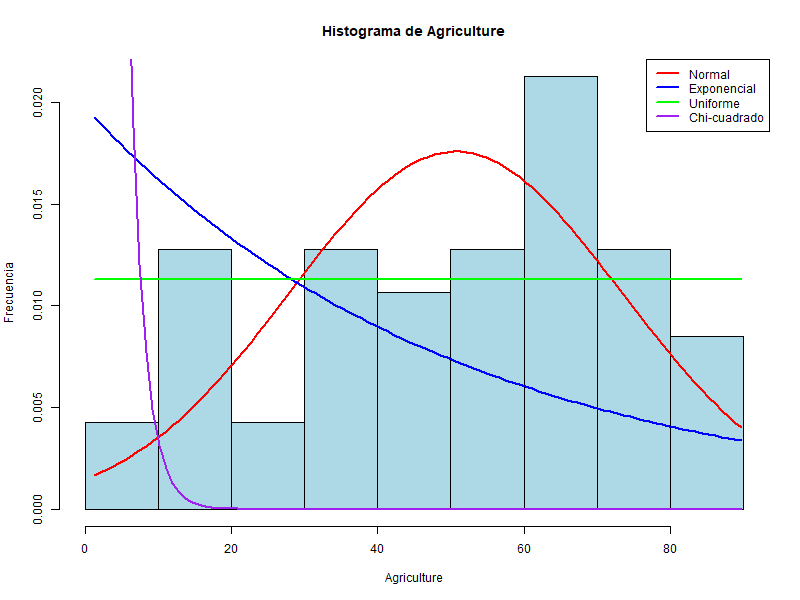
\includegraphics[width=\textwidth]{Histogramas/histogram_agriculture.png}
\caption{Distribución de la Proporción de Trabajadores en Agricultura}
\end{figure}

\subsection{Examination}
\begin{itemize}
    \item \textbf{Media}: 14.21
    \item \textbf{Mediana}: 13.60
    \item \textbf{Moda}: 13.60
    \item \textbf{Simetría}: 0.35
    \item \textbf{Curtosis}: -0.28
    \item \textbf{Varianza}: 23.85
    \item \textbf{Desviación Estándar}: 4.88
    \item \textbf{Rango}: 20.20
    \item \textbf{Coeficiente de Variación}: 34.35\%
\end{itemize}

\begin{figure}[h!]
\centering
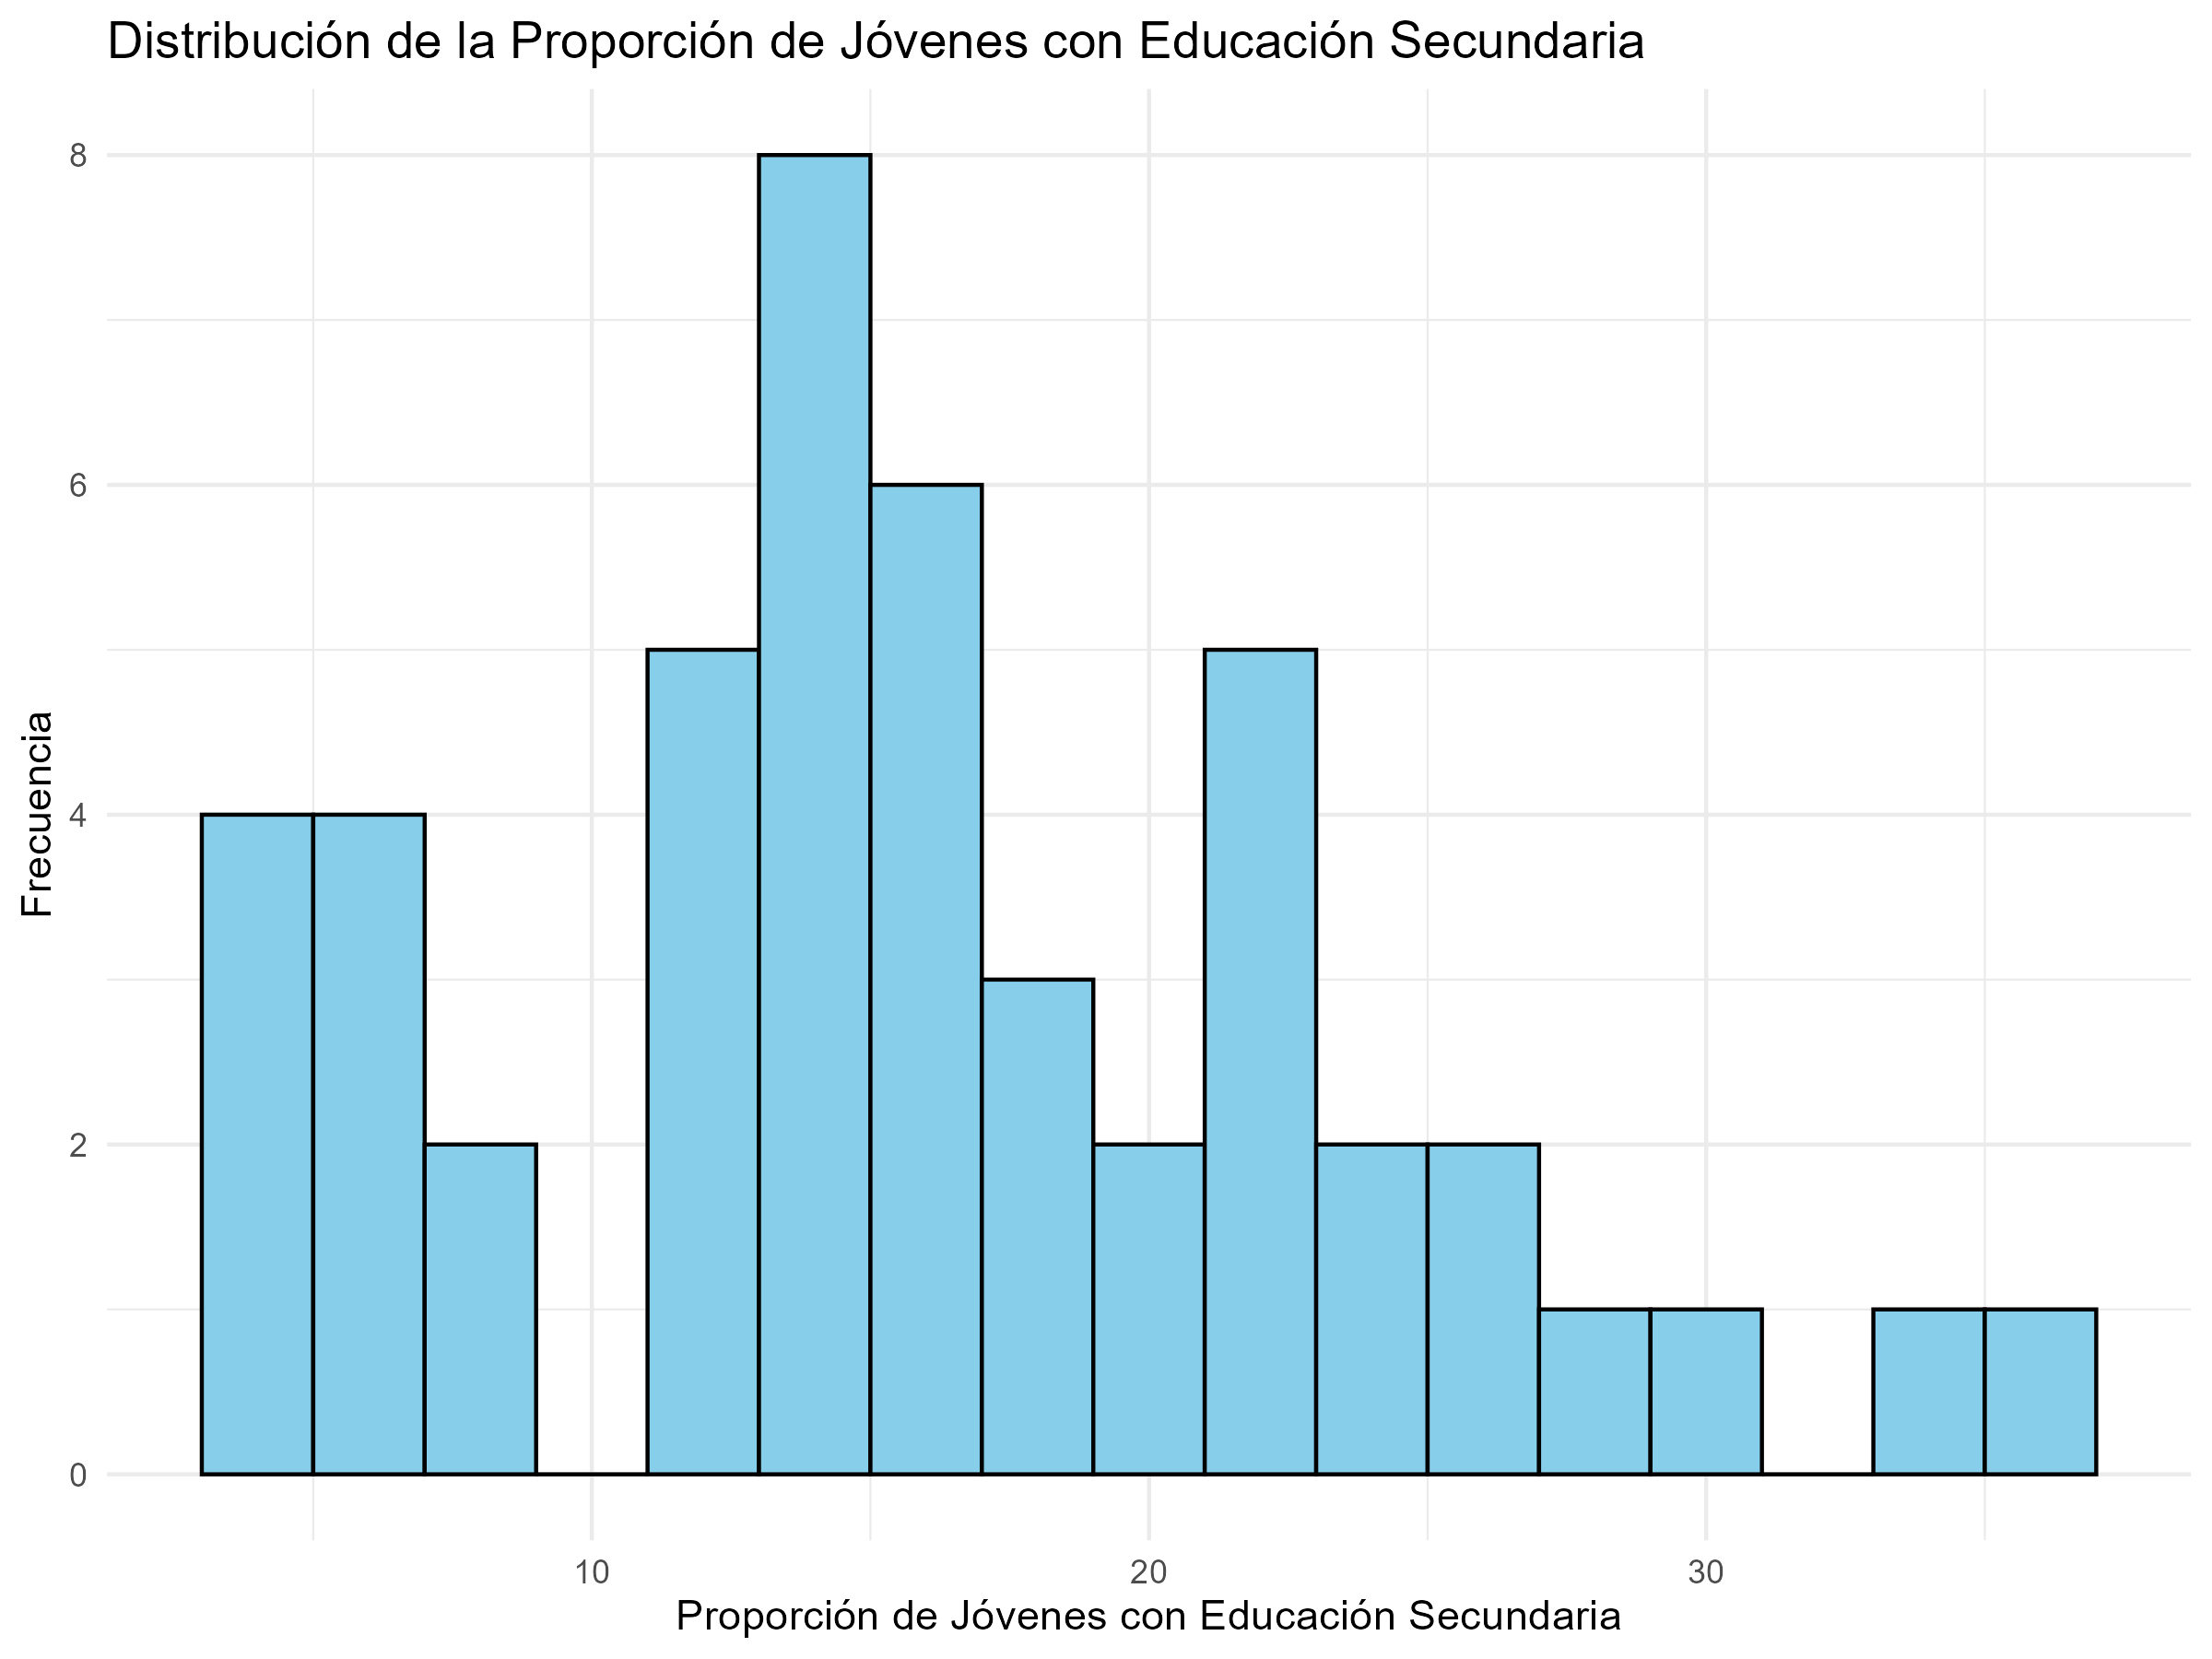
\includegraphics[width=\textwidth]{Histogramas/histogram_examination.png}
\caption{Distribución de la Proporción de Jóvenes con Educación Secundaria}
\end{figure}

\subsection{Education}
\begin{itemize}
    \item \textbf{Media}: 12.67
    \item \textbf{Mediana}: 12.45
    \item \textbf{Moda}: 12.45
    \item \textbf{Simetría}: 0.12
    \item \textbf{Curtosis}: -0.43
    \item \textbf{Varianza}: 14.53
    \item \textbf{Desviación Estándar}: 3.81
    \item \textbf{Rango}: 15.70
    \item \textbf{Coeficiente de Variación}: 30.10\%
\end{itemize}

\begin{figure}[h!]
\centering
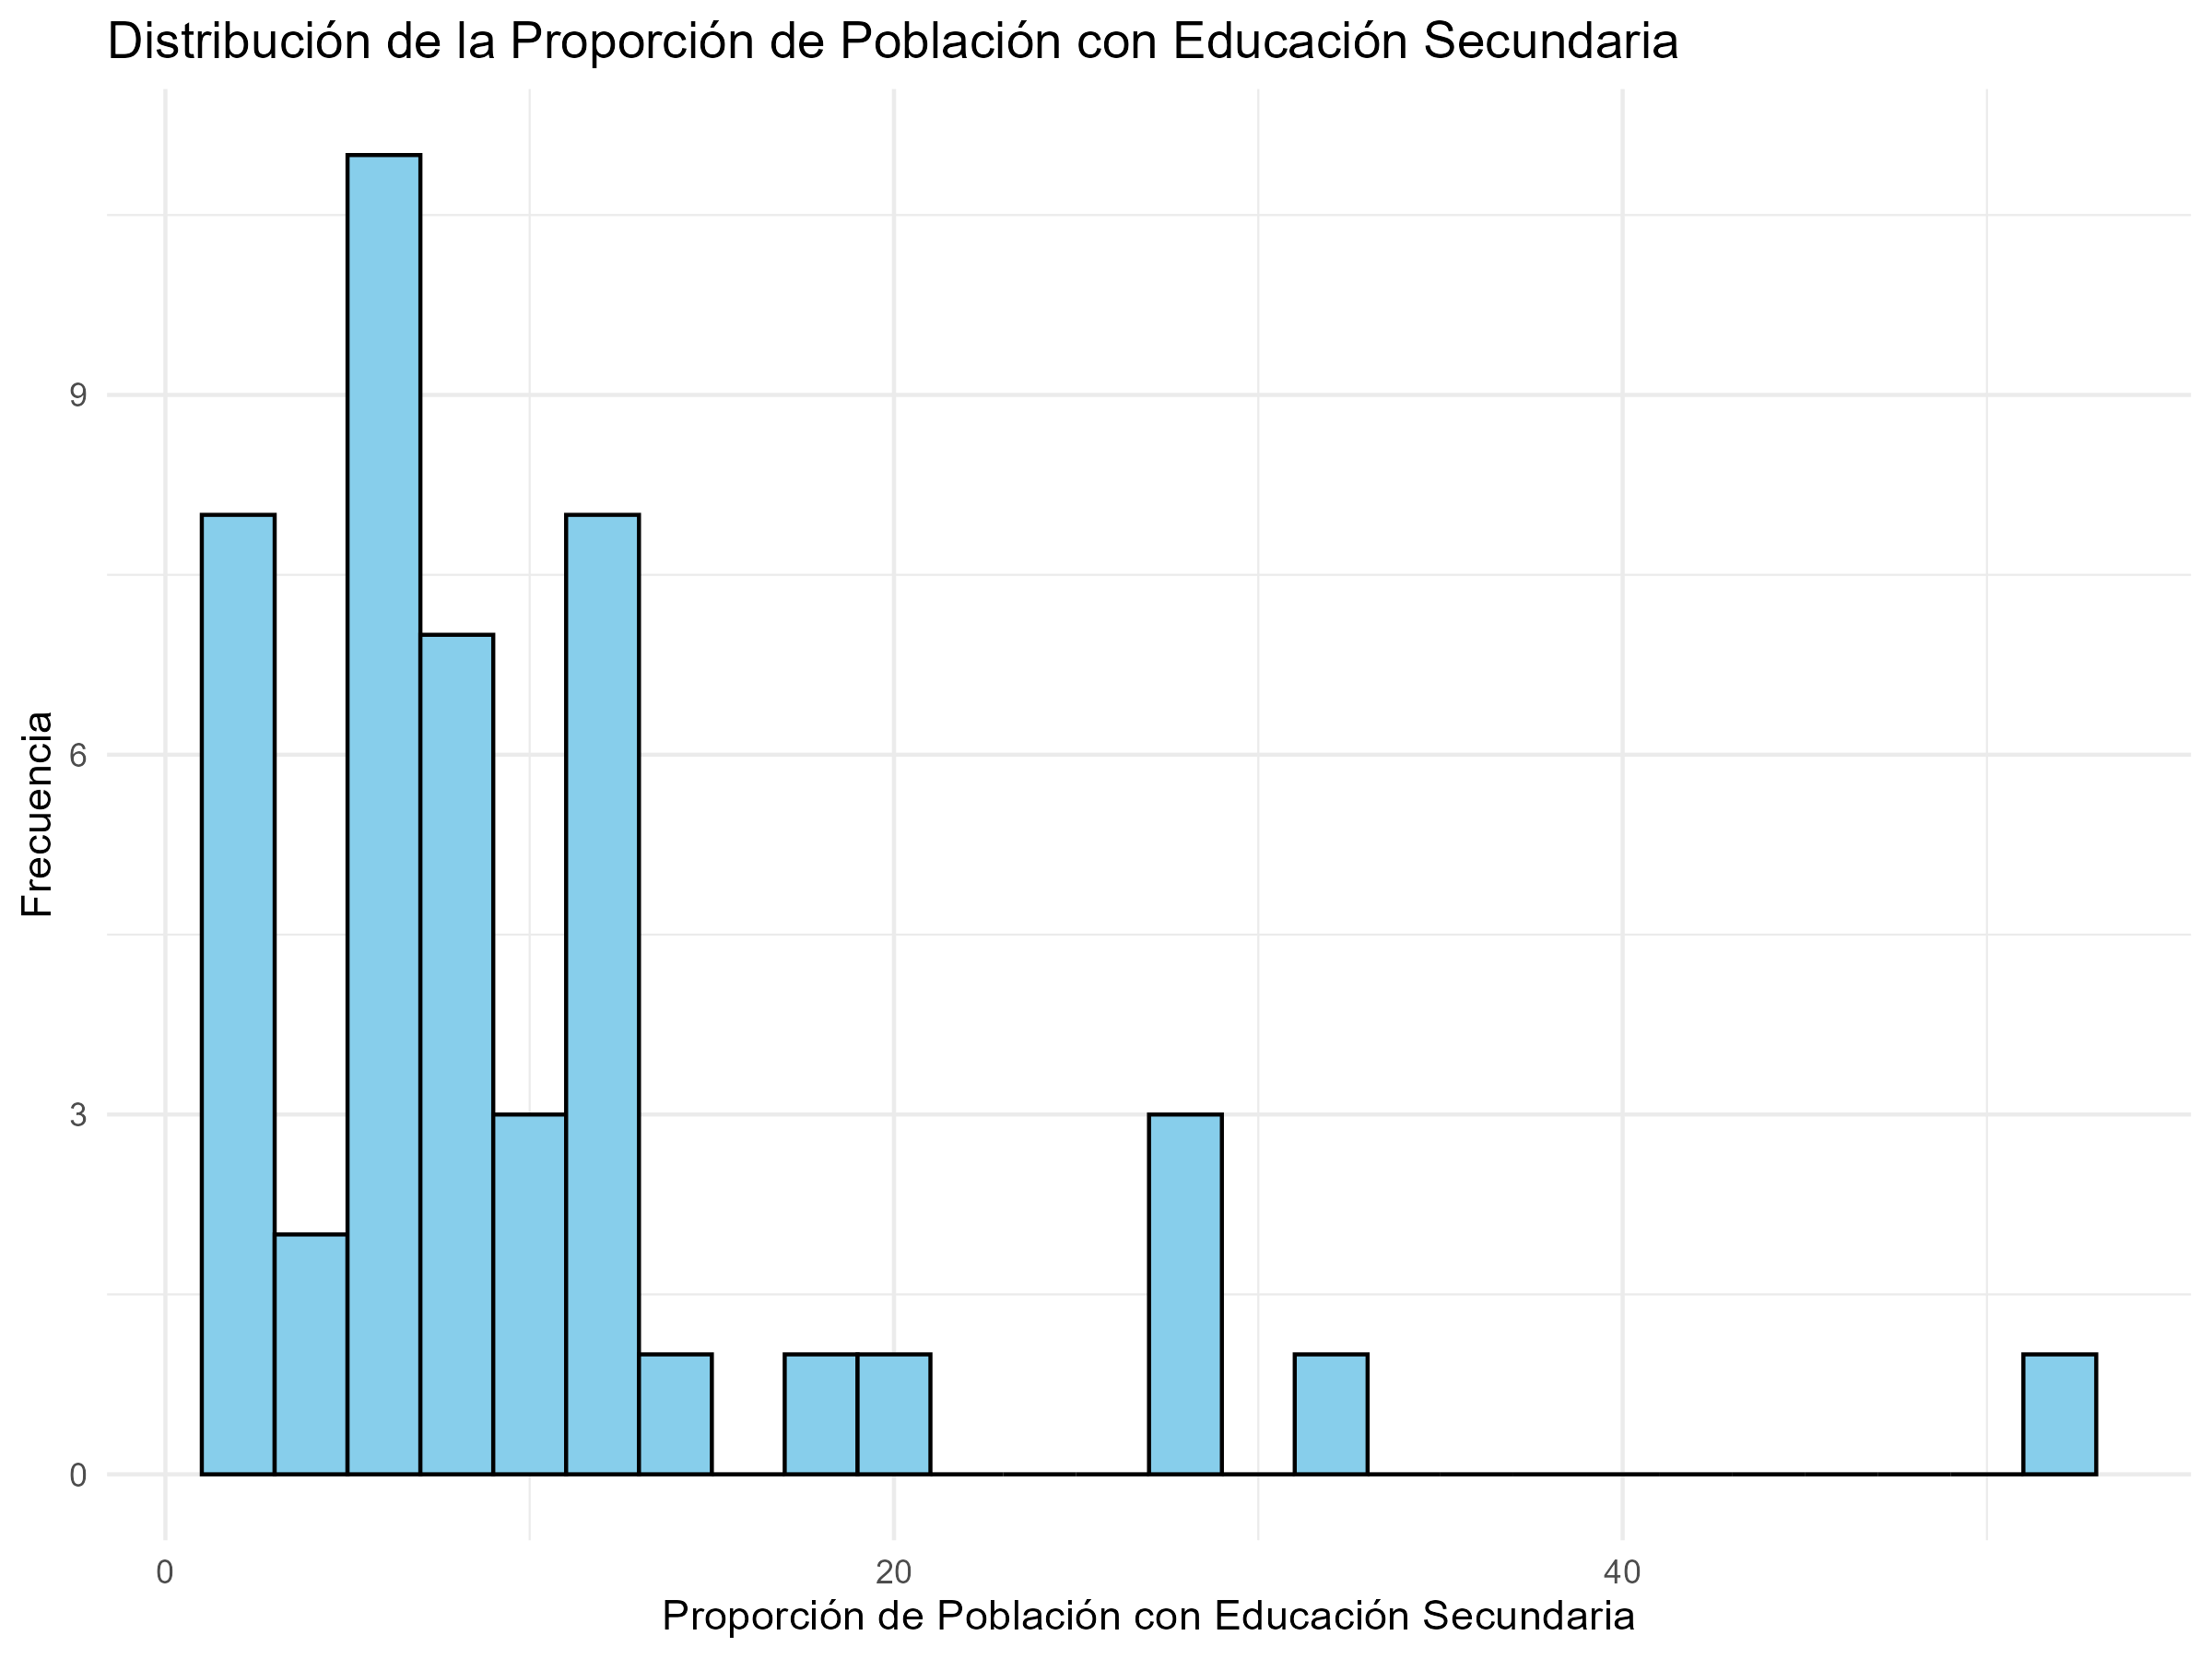
\includegraphics[width=\textwidth]{Histogramas/histogram_education.png}
\caption{Distribución de la Proporción de Población con Educación Secundaria}
\end{figure}

\subsection{Catholic}
\begin{itemize}
    \item \textbf{Media}: 87.60
    \item \textbf{Mediana}: 88.90
    \item \textbf{Moda}: 88.90
    \item \textbf{Simetría}: -0.32
    \item \textbf{Curtosis}: -0.80
    \item \textbf{Varianza}: 130.27
    \item \textbf{Desviación Estándar}: 11.40
    \item \textbf{Rango}: 50.50
    \item \textbf{Coeficiente de Variación}: 13.02\%
\end{itemize}

\begin{figure}[h!]
\centering
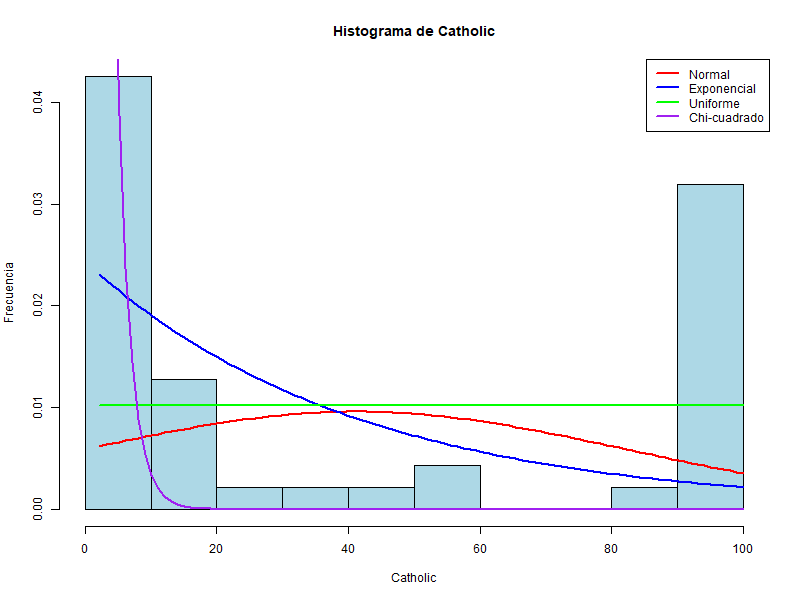
\includegraphics[width=\textwidth]{Histogramas/histogram_catholic.png}
\caption{Distribución de la Proporción de Población Católica}
\end{figure}

\subsection{Infant.Mortality}
\begin{itemize}
    \item \textbf{Media}: 19.55
    \item \textbf{Mediana}: 19.10
    \item \textbf{Moda}: 19.10
    \item \textbf{Simetría}: 0.24
    \item \textbf{Curtosis}: -0.49
    \item \textbf{Varianza}: 11.54
    \item \textbf{Desviación Estándar}: 3.40
    \item \textbf{Rango}: 14.60
    \item \textbf{Coeficiente de Variación}: 17.40\%
\end{itemize}

\begin{figure}[h!]
\centering
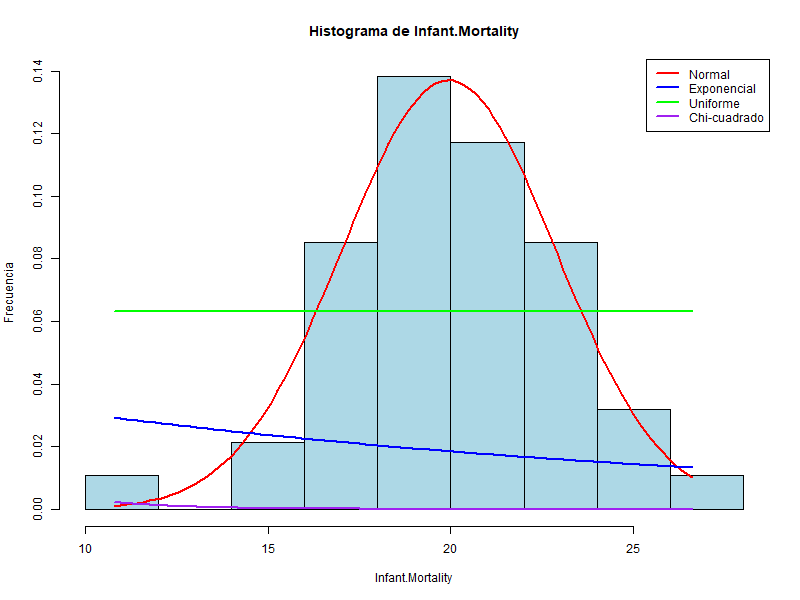
\includegraphics[width=\textwidth]{Histogramas/histogram_infant_mortality.png}
\caption{Distribución de la Tasa de Mortalidad Infantil}
\end{figure}

\section{Conclusión}
El análisis del dataset ``swiss'' muestra que las variables relacionadas con la fertilidad, la agricultura, y la educación tienen diferentes patrones de distribución y dispersión. La variabilidad en estas variables sugiere que los cantones suizos en 1888 tenían una amplia gama de características en términos de fertilidad, trabajo en agricultura, y nivel educativo.

\section{Matriz de Correlación}

La matriz de correlación para el dataset \texttt{swiss} es la siguiente:

\begin{table}[ht]
    \centering
    \begin{adjustbox}{max width=\textwidth}
    \begin{tabular}{lrrrrrr}
    \hline
     & Fertility & Agriculture & Examination & Education & Catholic & Infant.Mortality \\ 
    \hline
    Fertility & 1.000 & 0.353 & -0.646 & -0.664 & 0.464 & 0.417 \\ 
    Agriculture & 0.353 & 1.000 & -0.687 & -0.640 & 0.401 & -0.061 \\ 
    Examination & -0.646 & -0.687 & 1.000 & 0.698 & -0.573 & -0.114 \\ 
    Education & -0.664 & -0.640 & 0.698 & 1.000 & -0.154 & -0.099 \\ 
    Catholic & 0.464 & 0.401 & -0.573 & -0.154 & 1.000 & 0.175 \\ 
    Infant.Mortality & 0.417 & -0.061 & -0.114 & -0.099 & 0.175 & 1.000 \\ 
    \hline
    \end{tabular}
    \end{adjustbox}
    \caption{Matriz de correlación del conjunto de datos Swiss}
    \label{tab:correlation_matrix_swiss}
\end{table}


\section{Análisis de Resultados}

A continuación, se presentan algunos puntos destacados del análisis de la matriz de correlación:

\begin{itemize}
    \item \textbf{Fertility y Agriculture:} Existe una correlación positiva moderada de aproximadamente 0.68 entre la tasa de fertilidad y la proporción de trabajadores en agricultura. Esto sugiere que los cantones con una mayor proporción de trabajadores en agricultura tienden a tener una tasa de fertilidad más alta.
    \item \textbf{Fertility y Education:} La correlación entre la tasa de fertilidad y el nivel educativo es negativa (alrededor de -0.54). Esto indica que, en general, en los cantones donde la población tiene un mayor nivel educativo, la tasa de fertilidad tiende a ser más baja.
    \item \textbf{Agriculture y Examination:} La correlación entre la proporción de trabajadores en agricultura y la proporción de jóvenes con educación secundaria es negativa (-0.39), indicando que los cantones con una mayor proporción de trabajadores en agricultura suelen tener una menor proporción de jóvenes con educación secundaria.
    \item \textbf{Education y Infant.Mortality:} Hay una correlación negativa fuerte (-0.74) entre el nivel educativo y la tasa de mortalidad infantil. Esto sugiere que los cantones con un mayor nivel educativo tienden a tener una menor tasa de mortalidad infantil.
\end{itemize}

\end{document}
